\chapter{\acs{FELIX} project}

The first goal of the \acs{FELIX} project is to replace diverse, custom-made hardware readout solutions with a unified platform that relies on \acf{COTS} components. With this approach, tasks once handled by such custom hardware are now managed by software modules that subscribe to \acs{FELIX} cards inside off-the-shelf servers.

From an architectural perspective, \acs{FELIX} is built around a custom \acs{PCIe} card installed in a host server. Incoming data from detector front-ends reaches system memory via \acf{DMA}. Software on the host then distributes these data streams to network-connected clients.\\
Bidirectional communication is supported, allowing data to flow from software back to the front-end electronics. The \texttt{netio3} network library allows using TCP/IP if needed, in addition to \acf{RoCE} as a supported network protocol. This chapter examines the \acs{FELIX} project covering its hardware, firmware and software design.

\clearpage
\section{Hardware}

Three hardware implementations are currently relevant:

\begin{itemize}
    \item \textbf{FLX-182}: used for prototyping and testing new features;
    
    \item \textbf{FLX-155}: candidate card for \acs{ATLAS} Phase-II operations and an upgrade over FLX-182;
    
    \item \textbf{FLX-712}: older version developed for Phase-I, used in production, but no longer under development or used for testing new features.
\end{itemize}

\subsection{FLX-182}

The FLX-182 \cite{Ilic:2873569} (Figure \ref{fig:FLX-182-combined}) is a Phase-II prototype card developed by \acf{BNL}. It features:

\begin{itemize}
    \item AMD Versal Prime VP-1802 \acf{SoC}
    \item FireFly optical transceivers supporting up to 24 duplex links at 25 Gb/s \cite{firefly-optical-transceiver}
    \item \acf{LTI} interface (Figure~\ref{fig:ALTI} shows the \acs{ATLAS} \acl{LTI})
    \item Electrical trigger interface
    \item \acs{PCIe} Gen4 connectivity
\end{itemize}

\begin{figure}[htbp]
\centering
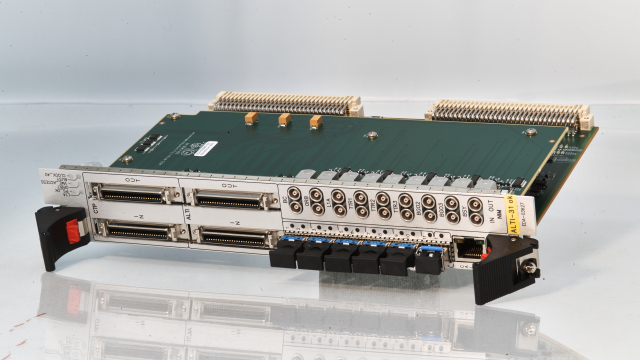
\includegraphics[width=\textwidth]{images/felix/lti.jpg}
\caption[ATLAS Local Trigger Interface]{The ATLAS \acl{LTI} is a replacement of the legacy \acf{TTC}.\\ \texttt{Timing}: Distribution of the \acs{LHC} bunch clock (the same clock source for entire system).\\\texttt{Trigger}: Decision from the trigger system indicating whether the data for a given event should be sent to the readout.\\ \texttt{Control}: Sends synchronization/configuration commands, subdetectors raise a Busy signal to indicated that the internal buffers are filling up.\\Image source \protect\cite{alti}.}
\label{fig:ALTI}
\end{figure}

This card requires a 16-lane \acs{PCIe} slot (preferably Gen4) configured with x8x8 bifurcation. Power is supplied through a \acs{PCIe} 6+2 pin cable, and the card's form factor necessitates two adjacent \acs{PCIe} slots for bracket installation. 
The operating system is PetaLinux. The OS and the \acl{PL} image for the \acs{FPGA} are embedded into a micro-SD card. The \acs{PL} can be reprogrammed by either updating the SD card contents or using the onboard \ac{JTAG} controller, accessible via the USB-C port on the front panel.

\begin{figure}[H]
\centering
\begin{subfigure}[b]{0.48\textwidth}
    \centering
    \includegraphics[width=\textwidth]{images/felix/felix-front-panel.png}
    \caption{FLX-182 front panel.}
    \label{fig:FLX-182-panel}
\end{subfigure}
\hfill
\begin{subfigure}[b]{0.48\textwidth}
    \centering
    \includegraphics[width=\textwidth]{images/felix/FLX-182.png}
    \caption{FLX-182 top view.}
    \label{fig:FLX-182}
\end{subfigure}
\caption{FLX-182 hardware.}
\label{fig:FLX-182-combined}
\end{figure}

\subsection{FLX-155}
\label{subsec:FLX-155}
The FLX-155 (Figure \ref{fig:FLX-155}) is the designated candidate for \acs{ATLAS} Phase-II operations, with advancement over the FLX-182 prototype like the support for a more recent \acs{PCIe} standard, and double the number of optical transceiver links. Its specifications include:

\begin{itemize}
    \item AMD Versal Premium VP-1552 SoC
    \item Support for up to 48 duplex links rated at up to 25 Gb/s via FireFly optical transceivers
    \item \acs{PCIe} Gen5 connectivity
    \item \acs{LTI} interface via a dedicated FireFly B04 module
    \item Optional 400 GbE interface capability (not utilized in ATLAS)
\end{itemize}

The FLX-155 will be 1cm shorter than the FLX-182 and will require similar installation parameters: a 16-lane \acs{PCIe} slot (preferably Gen5) with x8x8 bifurcation configuration. At least one \acs{PCIe} 6+2 pin power cable is required. Like its predecessor, the FLX-155 is equipped with an SD card containing both the PetaLinux operating system and \acl{PL} images.

\begin{figure}[H]
\centering
\begin{subfigure}[b]{0.7\textwidth}
    \centering
    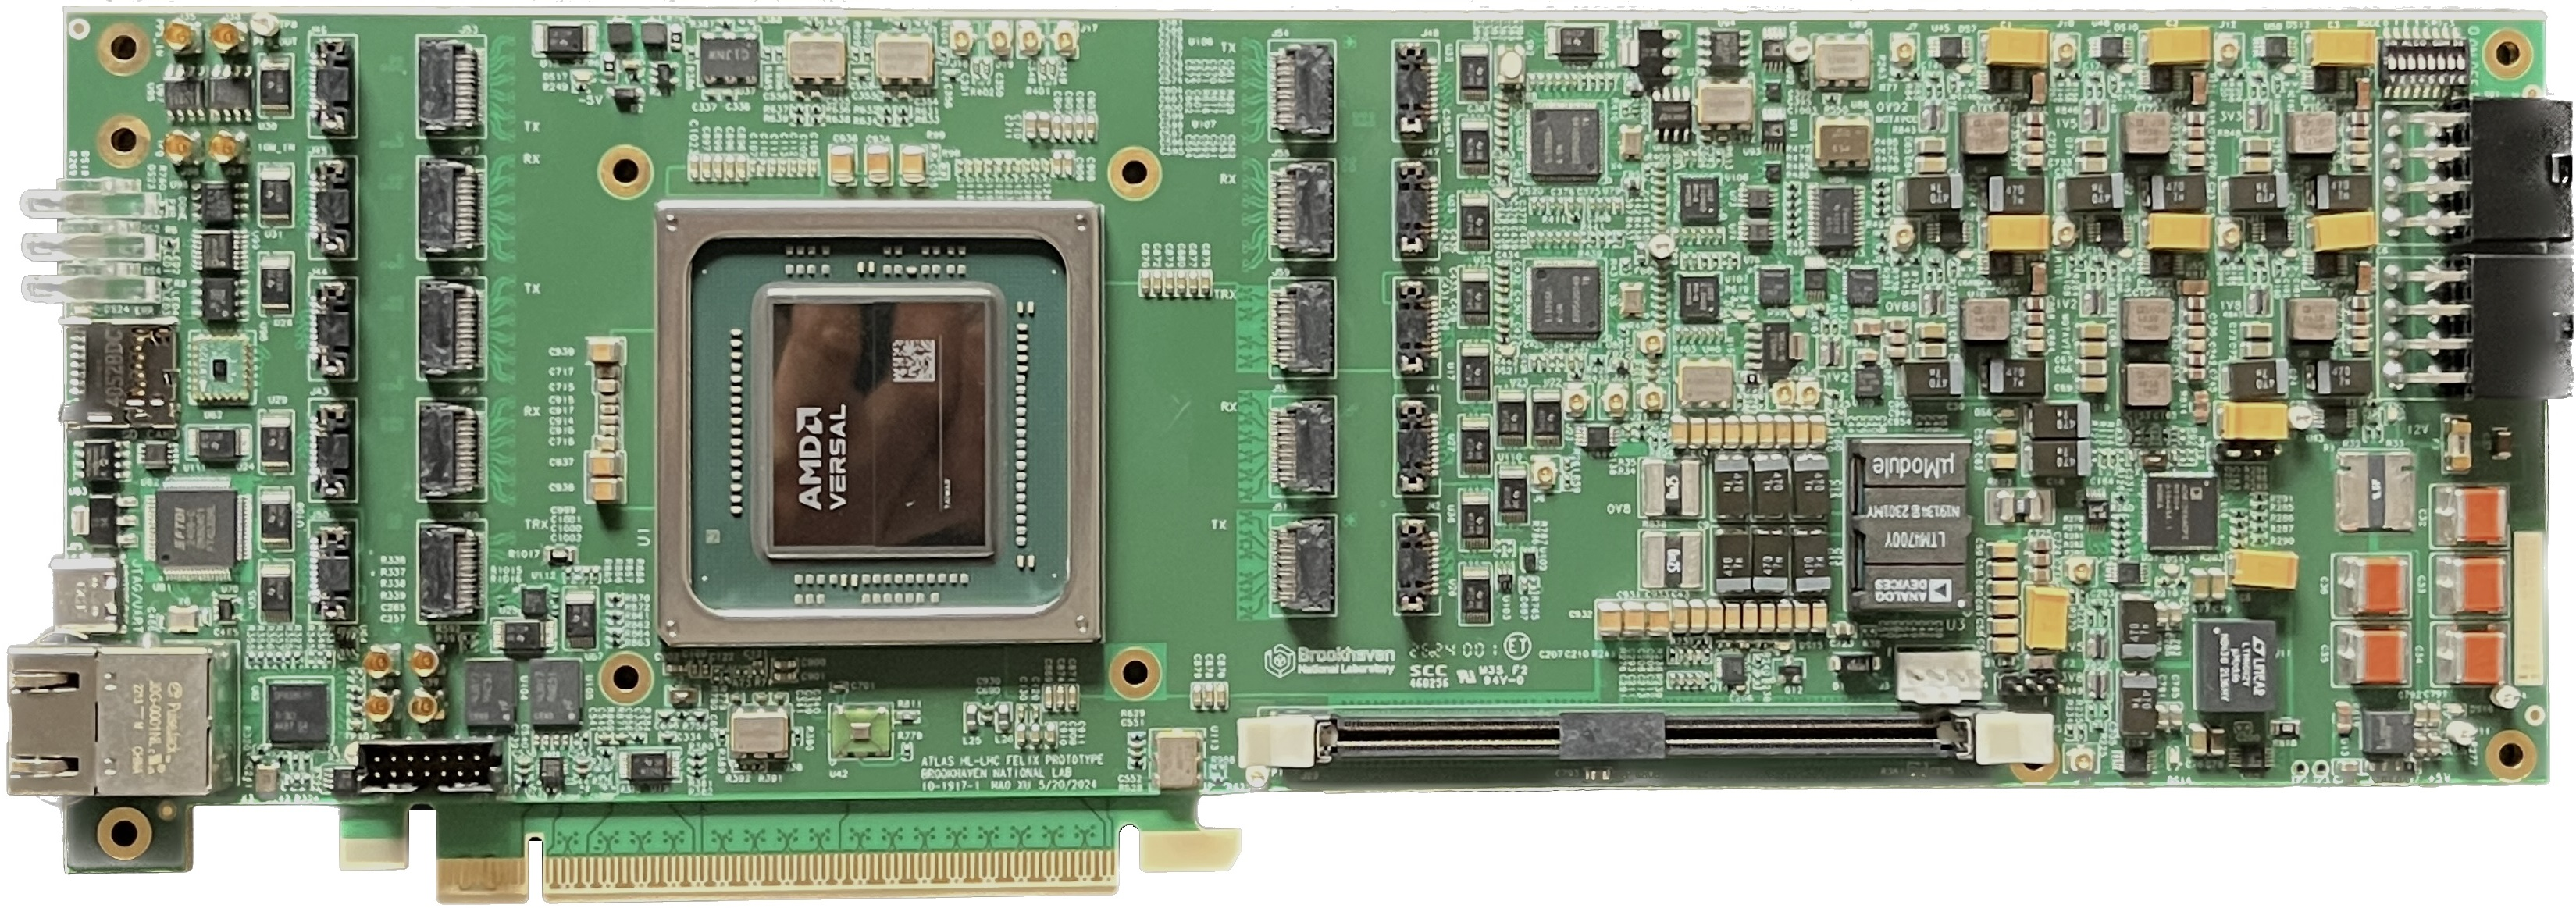
\includegraphics[width=\textwidth]{images/felix/flx155_top.jpg}
    \caption{FLX-155 front view.}
    \label{fig:FLX-155-top}
\end{subfigure}

\vspace{0.2cm}

\begin{subfigure}[b]{0.7\textwidth}
    \centering
    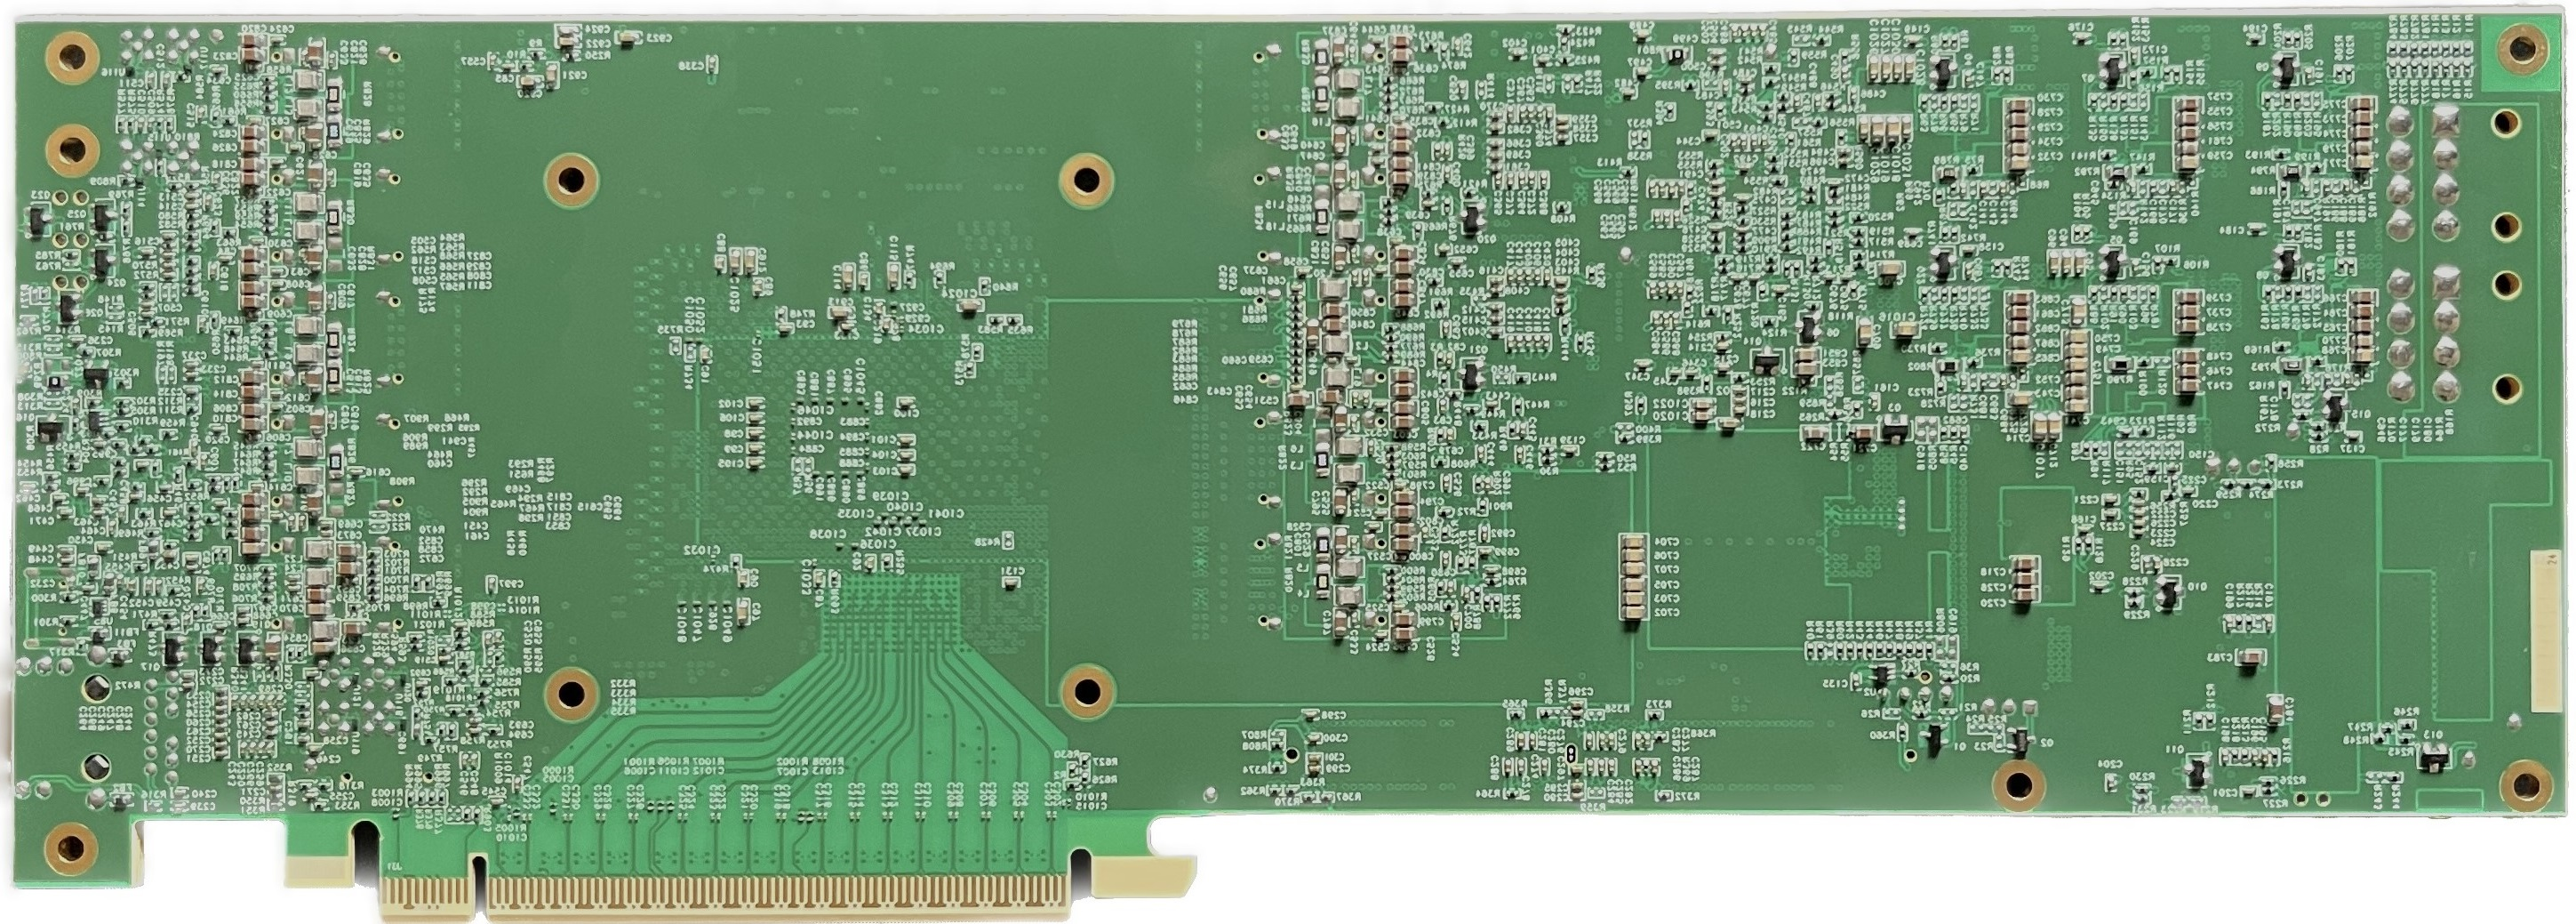
\includegraphics[width=\textwidth]{images/felix/flx155_bot.jpg}
    \caption{FLX-155 rear view.}
    \label{fig:FLX-155-bot}
\end{subfigure}
\caption{FLX-155 hardware.}
\label{fig:FLX-155}
\end{figure}

\clearpage
\section{Firmware}
\label{sec:felix-firmware}

The \acs{FELIX} firmware handles physical layer connectivity, data buffering, and communication with the host through the \ac{PCIe} interface. There are different firmware "flavours" that are used depending on what \acl{FE} is using the \acs{FELIX} card.\\
Below is a comprehensive list of all the firmware types depending on the protocol the \acs{FELIX} card needs to communicate with.

\subsection{\acl{GBT} and Versatile Link}
\label{subsec:felix-gbt}

The \ac{GBT} chipset, combined with the Versatile Link optical technology \cite{gbt-versatile-link}, have evolved from \ac{CERN}'s Radiation Hard Optical Link Project. Versatile Link is a radiation-tolerant bi-directional optical link for data transfer among \acs{GBT} endpoints. The \ac{GBT} protocol aggregates lower-bandwidth logical links (\acs{E-link}s) from front-end devices into a single link operating at up to 5~Gb/s.

\begin{definition}
\label{def:elink}
An \acs{E-link} is a virtual lane inside a physical optical link. By using multiple \acs{E-link}s, it is possible to transmit multiple data streams in parallel.
\end{definition}

\begin{figure}[H]
\centering
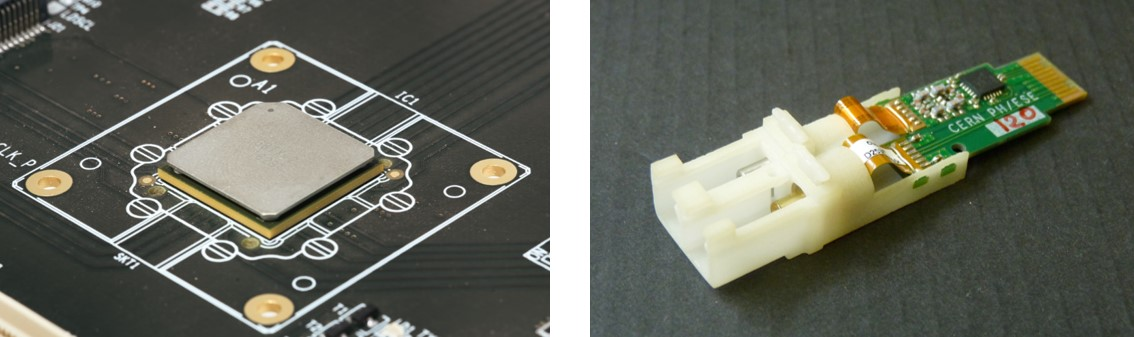
\includegraphics[width=\textwidth]{images/felix/gbt.jpg}
\caption[GBT and Versatile Link]{\acs{GBT} chip (left) and Versatile Link (right). Source \protect\cite{gbt-versatile-link}}
\label{fig:gbt-versalink-combined}
\end{figure}

\subsection{\acf{lpGBT}}
\label{subsec:felix-lpgbt}

The \acf{lpGBT} \cite{lpgbt} is an evolution of the \acf{GBT} project and is a radiation tolerant \acs{ASIC} that can be used to implement multipurpose high speed bidirectional optical links for high-energy physics experiment, with 2.56~Gb/s downlinks (readout to front-end) and 5.12~Gb/s or 10.24~Gb/s uplinks (front-end to readout), depending on the selected operation mode. The aim of \acs{lpGBT} is to allow a single bidirectional link to be used simultaneously for data readout, trigger data, timing, experiment control and monitoring.

\begin{figure}[H]
\centering
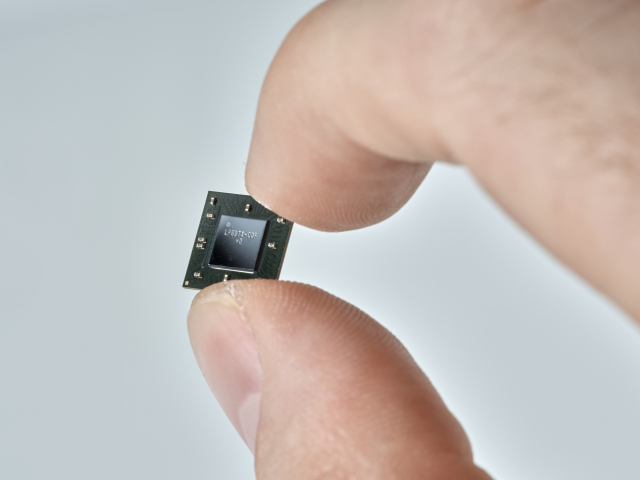
\includegraphics[width=\textwidth]{images/felix/lpgbt.jpg}
\caption[lpGBT chip]{\acs{lpGBT} chip. Source \protect\cite{lpgbt-image-source}}
\label{fig:lpgbt}
\end{figure}

\subsection{FULL Mode}
\label{subsec:felix-fullmode}

The FULL mode protocol \cite{fullmode} is used for \acl{FE} electronics with no radiation constraints, and it requires less \acs{FPGA} resources compared to \acs{GBT}. FULL mode provides a single, wide data stream without using the \acs{E-link} substructures or the handshaking mechanisms in \acs{GBT}/\acs{lpGBT}, and allows a data rate of 9.6~Gb/s. After 8b/10b encoding, this yields a peak uplink payload of 7.68~Gb/s.\\
Downstream traffic at 9.6~Gb/s transmits timing signals (such as the 40.079~MHz \acs{LHC} clock) and control data from the \acf{LTI}.\\
Early releases of FULL mode reused GBT-compatible downlinks for legacy \acf{TTC} messaging.

\subsection{Interlaken Mode}
\label{subsec:felix-interlaken}

For even higher throughput, the firmware supports the Interlaken protocol \cite{InterlakenSpec} with link speeds as high as 25~Gb/s. Interlaken follows a structure similar to FULL mode, offering a single high-speed data channel without sub-channels. Downstream communication relies on a 9.6~Gb/s link and conveys \acs{LTI} messages equivalently to FULL mode.

\subsection{\acs{ATLAS} \acs{ITk} Pixel and Strip Compatibility}
\label{subsec:felix-itk}

\acf{ITk} \cite{atlas-itk-pixel-detector} is a new detector meant for Phase II \acs{ATLAS}.
A dedicated firmware has been developed to interface with  Pixel and Strip sub-detectors.\\

The \emph{Strip} flavour was designed to read out the \acs{ITk} Strip detector over \acs{lpGBT} with 8b/10b e-links.\\
The \emph{Pixel} flavour was designed to read out the \acs{ITk} Pixel detector over \acs{lpGBT} with Aurora \cite{aurora-protocol} e-links.\\

Aurora \cite{aurora-protocol} is a high-speed, link layer, serial communication protocol developed by Xilinx, which is used to transmit data between the \acs{FPGA} and the front-end electronics.

\clearpage
\section{Software}

All the software for the \acs{FELIX} project is open source and hosted on Gitlab under the name of felix-distribution \cite{felix-distribution}. This software is formally supported and built for systems using the AlmaLinux 9 \acl{OS}.

\subsection{\acs{FELIX} drivers}

\subsubsection{flx\_driver}

The \texttt{flx} driver~\cite{felix-driver} is a device driver developed for Linux for \acs{PCIe}-based hardware. It is responsible for detecting \acs{FELIX} cards, managing hardware interrupts, and exposing a set of \texttt{ioctl} interfaces for user-space interaction. Within the \acs{ATLAS} software framework, the \texttt{flx} driver is typically deployed in conjunction with the \texttt{cmem\_rcc} driver, and optionally, the \texttt{io\_rcc} driver, to provide support for cross-device communication and memory management.

\subsubsection{cmem\_rcc}

The allocation of contiguous memory buffers is a requirement for high-performance \acf{DMA} operations in general, and for data acquisition systems such as \acs{FELIX} in particular. In 2018, the standard \ac{CMA} was evaluated and found inadequate for \ac{FELIX} requirements, primarily due to limitations in support and documentation \cite{cmem-rcc}.

The cmem\_rcc \cite{cmem-rcc} package, well established within the \acs{ATLAS} experiment, was selected as the baseline solution. The cmem\_rcc driver and its associated user-space library is based on the kernel's \texttt{alloc\_pages\_node()} and \texttt{alloc\_pages()} system calls. These calls allow memory to be allocated either from a specific \ac{NUMA} node or without \ac{NUMA} awareness, providing flexibility for deployment on multi-socket systems.

cmem\_rcc supports two allocation strategies: (1) on-demand allocation of individual buffers, and (2) pre-allocation of a large contiguous memory region at driver load time, from which user applications can request fragments as needed.

The driver supports concurrency and synchronization, using spinlocks to ensure thread safety on \ac{SMP} systems \cite{cmem-rcc}.

\subsection{Felix Distribution}

Felix Distribution \cite{felix-distribution} is a repository in which all the \acs{FELIX}-related software is contained. As a logical consequence, \acs{FELIX} software is a collection of projects that are separately developed.\\
Below is a non-comprehensive list of components of Felix Distribution --- followed by a brief description --- focusing only on modules relevant to the thesis.

\textbf{elinkconfig}\\
The \texttt{elinkconfig} module is responsible for the configuration and management of \acs{E-link}s. This module provides utilities to enable and disable \acs{E-link}s define, modify, and query the settings of each \acs{E-link}.

\textbf{felix-bus-fs}\\
\texttt{felix-bus} translates \acs{FELIX} specific IDs (see Definition~\ref{def:FID}) into generic network information by exposing the information as files within the Linux file system. In the next chapter there will be a more detailed explanation of what \texttt{felix-bus} does (see Section~\ref{sec:felix_bus}).

\textbf{felix-star}\\
\texttt{felix-star} is the primary readout application. More on this module in the next chapter \emph{felix-star} (Chapter~\ref{chap:felix_star}).

\textbf{felix-client}\\
\texttt{felix-client} is the client application that \acs{FELIX} software users (like for example the Detector software developers) use to communicate with server applications of \texttt{felix-star}.

\textbf{felix-monitor}\\
The \texttt{felix-monitor} module is responsible for monitoring the status and performance of the \acs{FELIX} system. It collects and reports \acs{FELIX}-specific metrics, as well as more general ones like data throughput and error rates.

\textbf{flxcard}\\
The \texttt{flxcard} module is the user-space driver library of a \acs{FELIX card}, and serves as the primary hardware abstraction layer for the \acs{FELIX} \acs{PCIe} cards installed in the host system.

\textbf{ftools}\\
The \texttt{ftools} module comprises a suite of utility programs and scripts designed to perform common --- and often low-level --- tasks in the \acs{FELIX} environment, generally used for testing and debugging \acs{FELIX} dataflow and control operations including interaction with remote peers.

\textbf{netio3}\\
\texttt{netio3} will be expanded upon in the next chapter \emph{Netio3} (Chapter~\ref{chap:netio3}).

\clearpage
\section{Personal Contributions}

\subsection{Hardware Testing and Assembly}
\label{sec:felix-hardware-contributions}
The primary hardware contribution involved the testing (Figures~\ref{fig:felix-testing}, \ref{fig:bist}, \ref{fig:eyescan-test}) and assembly (Figure~\ref{fig:batch-felix-cards}) of the FLX-182-1B cards. I subjected the cards to a series of previously defined tests:

\begin{enumerate}
    \item \textbf{Component Verification}
    \begin{itemize}
        \item Visually inspected the most important discrete components (e.g. resistors, capacitors)
        \item Measured those components using a multimeter
    \end{itemize}

    \item \textbf{Power Management Configuration}
    \begin{itemize}
        \item Programmed the power delivery controller (ADM1266)
    \end{itemize}

    \item \textbf{FPGA Programming}
    \begin{itemize}
        \item Uploaded the programmable logic test firmware onto the FPGA and flash memory
    \end{itemize}

    \item \textbf{Mechanical Assembly}
    \begin{itemize}
        \item Assembled the fansink, \acs{PCIe} bracket, DDR module, and FireFly modules
        \item Installed a jumper on J40 (adjacent to fan power connector), connecting the top pin (GND) with the central pin. This sets the fan at maximum speed upon power-on
    \end{itemize}

    \item \textbf{FPGA Functionality Test}
    \begin{itemize}
        \item Prepared an SD card containing both the boot loader and the PetaLinux/BIST firmware
        \item Completed electrical and optical verification steps
    \end{itemize}

    \item \textbf{Front Panel Electrical Signals Test}
    \begin{itemize}
        \item Validated all front-panel electrical connections
    \end{itemize}
\end{enumerate}

\begin{figure}[H]
\centering
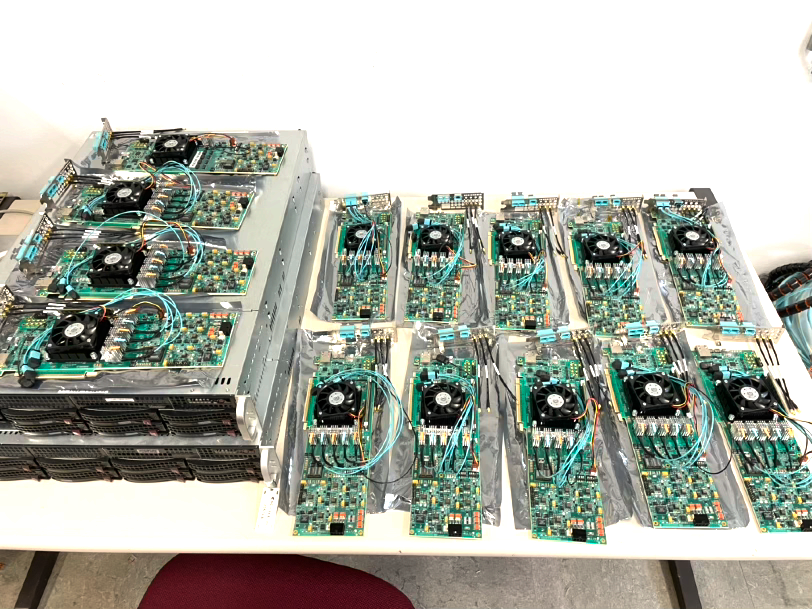
\includegraphics[width=\textwidth]{images/contributions/felix-cards.png}
\caption{A batch of fully tested and assembled FLX-182-1B cards.}
\label{fig:batch-felix-cards}
\end{figure}

\subsubsection{Tools}

The assembly of the cards required specialized equipment, and programming the power delivery controller was performed using an Aardvark I2C/SPI host adapter. The \acs{FPGA} was configured with Vivado \cite{vivado}. Electrical signal verification and validation of the front panel and active components involved the use of an oscilloscope, a power supply unit, and a function generator. Additionally, a server running with a \acs{DHCP} server was utilized to test the fiber connections, and a \acs{PCIe} loopback test card was employed to ensure proper \acs{PCIe} functionality.

\clearpage
\begin{figure}[htbp]
\begin{minipage}{0.9\textwidth}
\centering
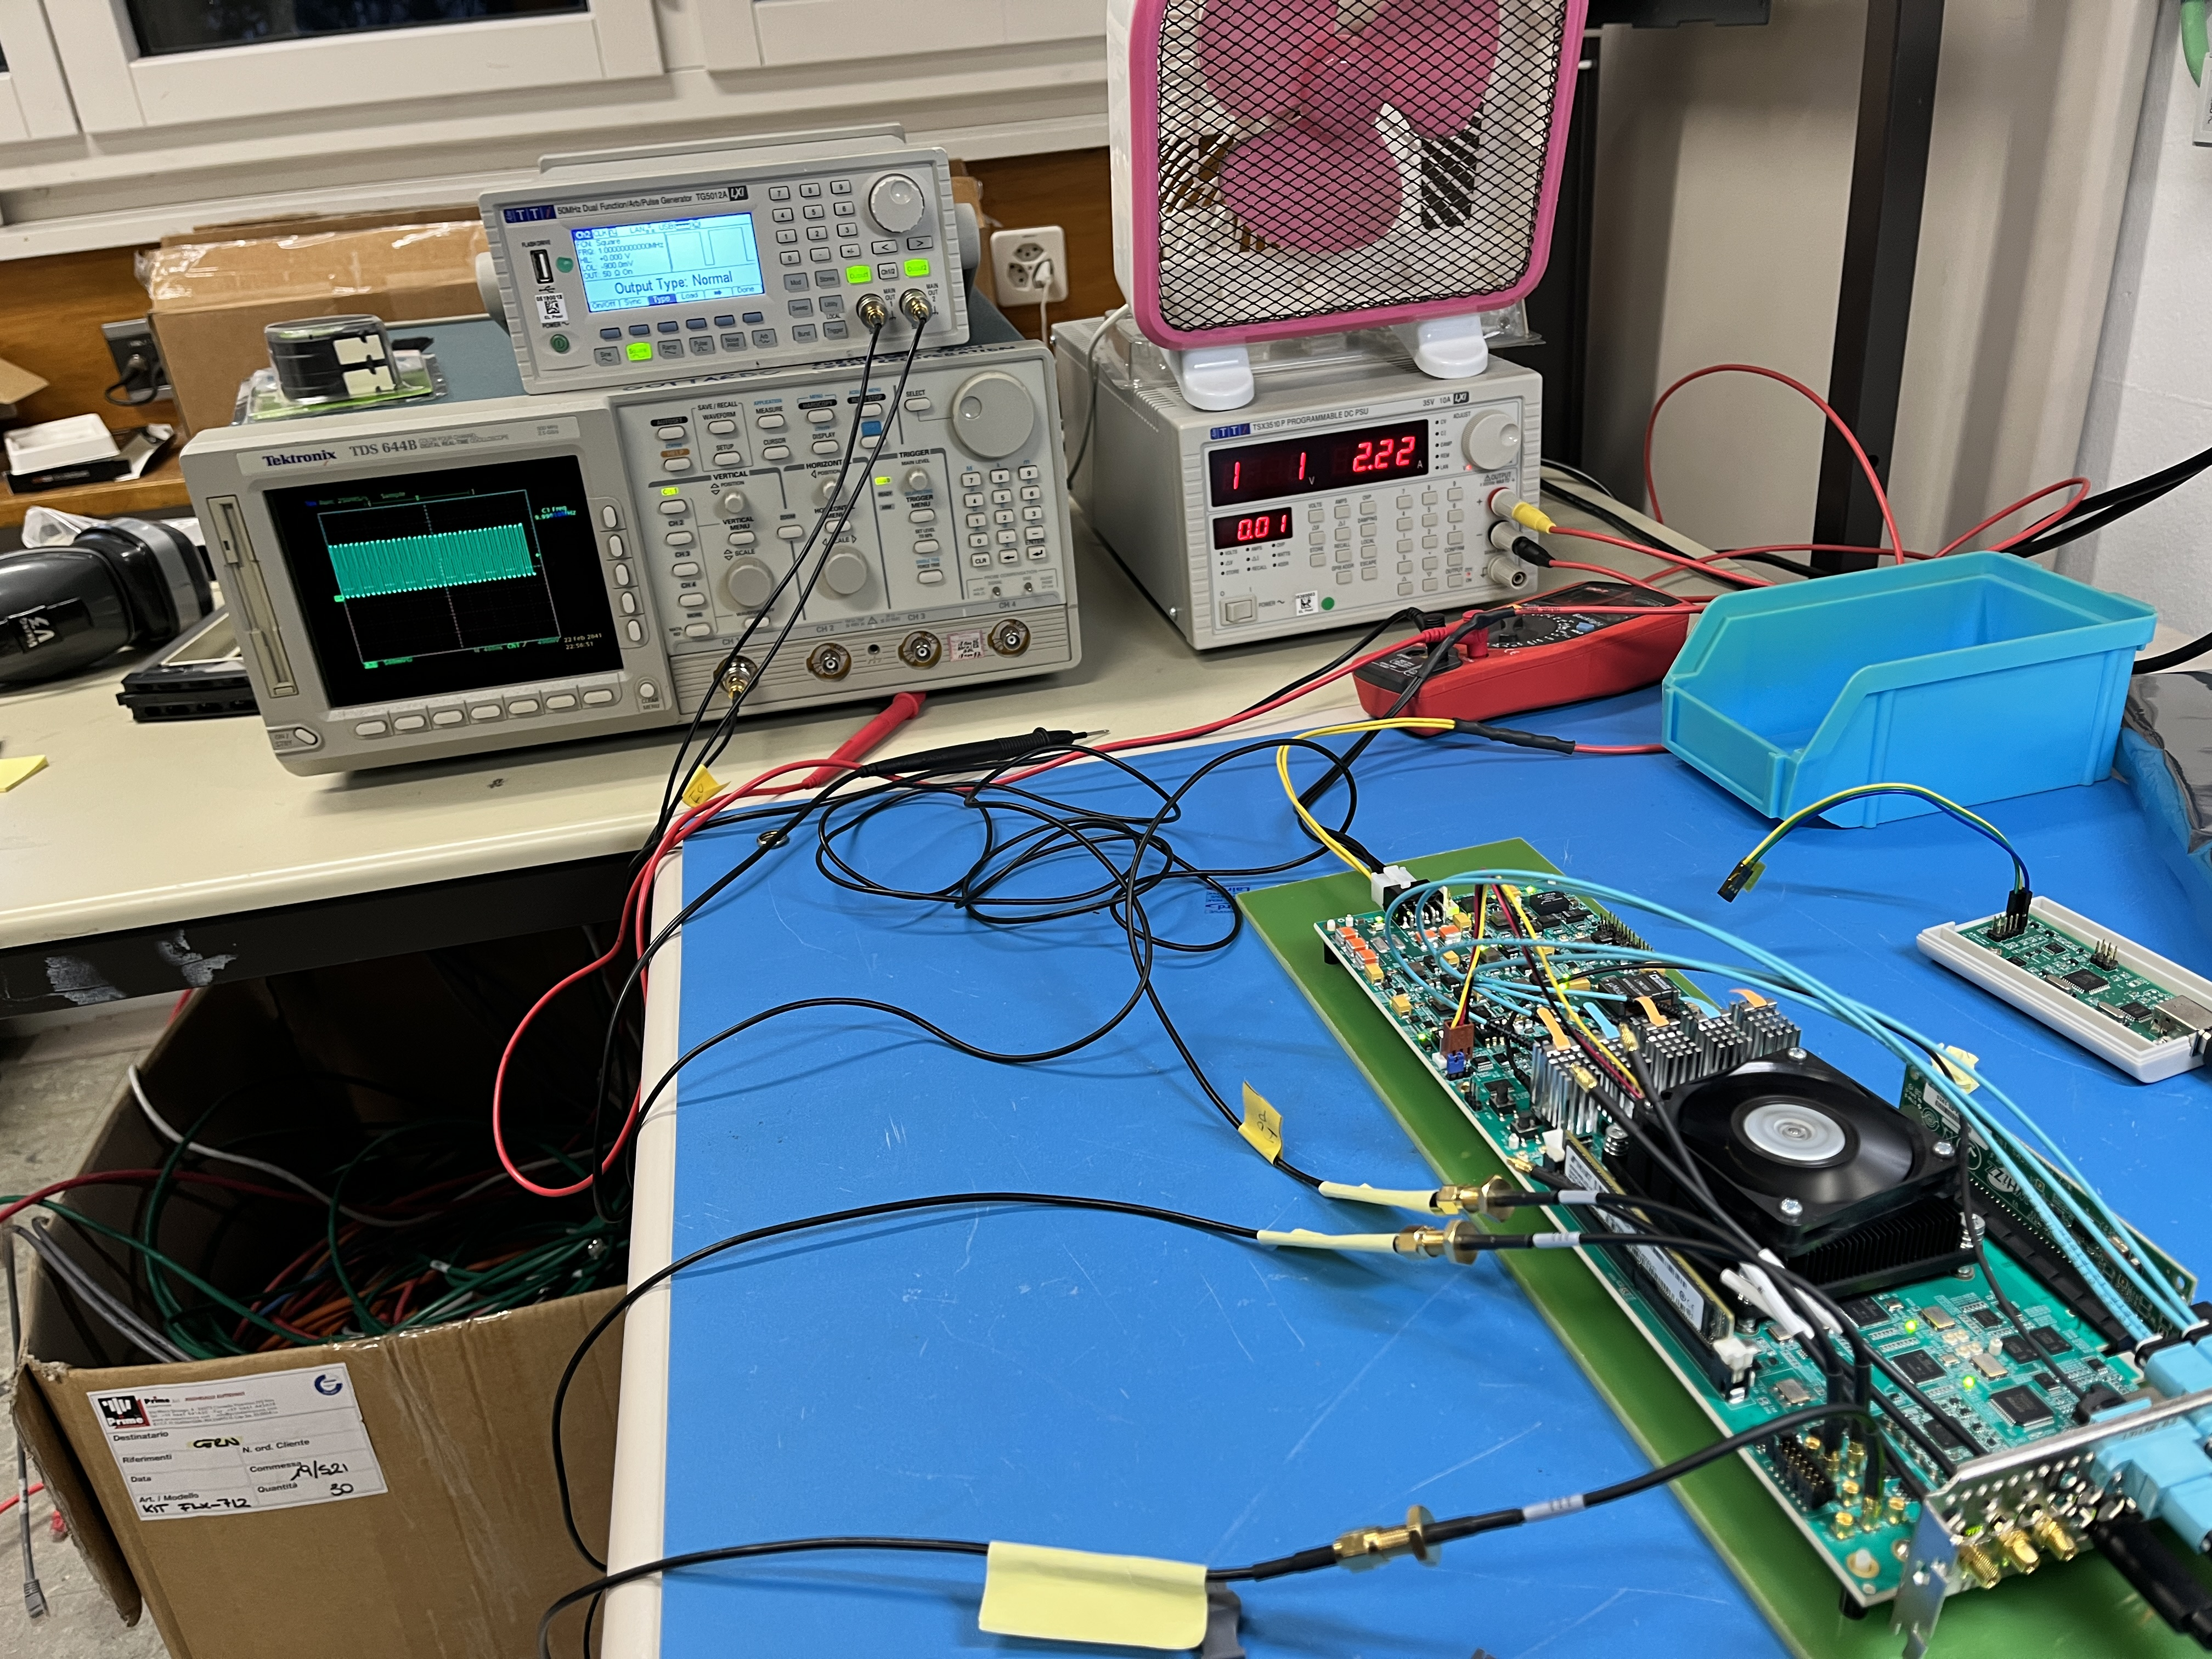
\includegraphics[width=0.8\textwidth]{images/contributions/felix-card-testing.jpg}
\caption[FELIX card testing setup]{Testing a \acs{FELIX} card. The PSU on the right, with a fan on top to help cool the \acs{FPGA}. Also on the right detached the Aardvark host adapter. The function generator is on top of the oscilloscope, with the probes attached to the electrical triggers. The \acs{PCIe} loopback scan is barely visible behind the aquamarine-colored fiber-optic cables, just on top of the mounted fan. What is not visible is the fibers connecting in a loopback the Firefly \protect\cite{firefly-optical-transceiver} optical transceiver modules, the \acs{JTAG} and UART cables.}
\label{fig:felix-testing}
\end{minipage}\hfill
\begin{minipage}{0.9\textwidth}
\centering
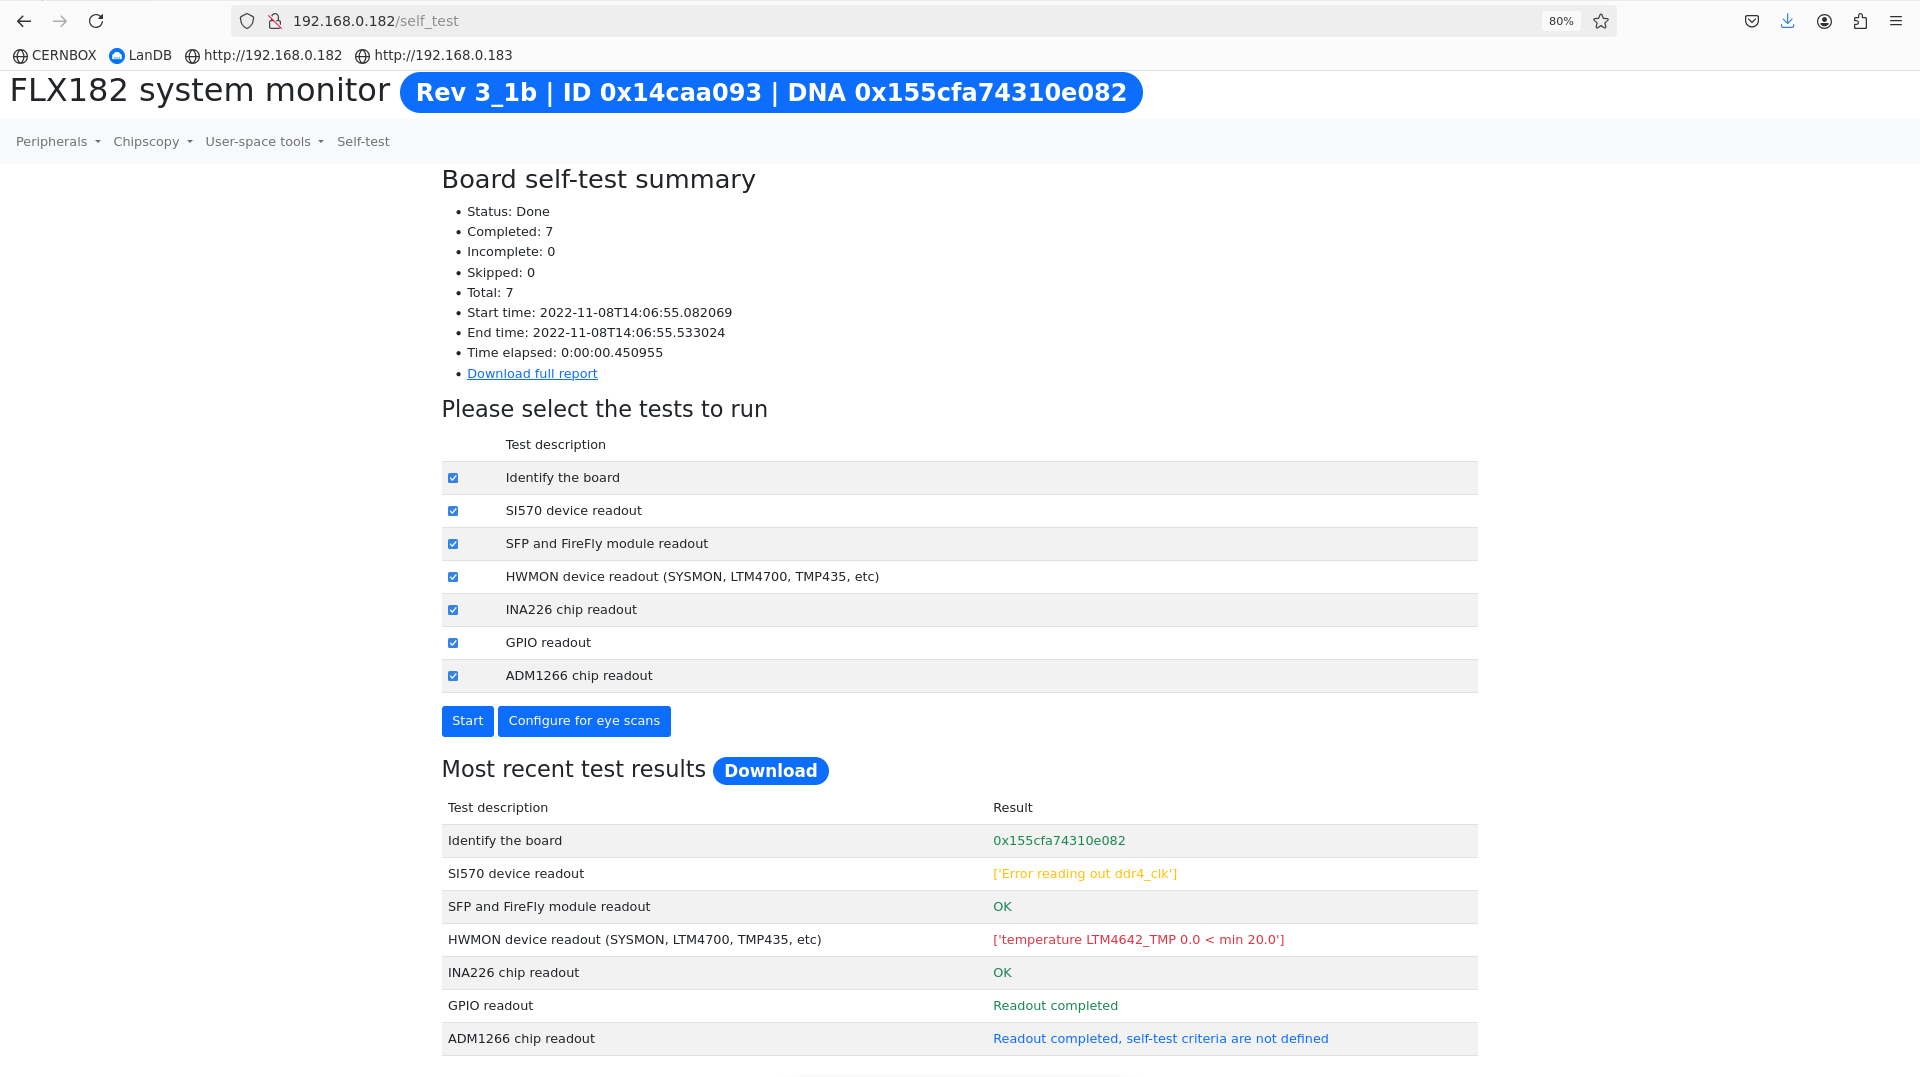
\includegraphics[width=\textwidth]{images/contributions/BIST.png}
\caption[Builtin Selftest screenshot]{Builtin Selftest. The \acs{DHCP} server is needed to give an IP to the card; an Ethernet cable connects the card to the server. The \acs{FELIX} card exposes this website which allows to check if all the active components in the \acs{PCB} are reachable and prepares the card for the eyescan test.}
\label{fig:bist}
\end{minipage}
\end{figure}

\begin{figure}[H]
\centering
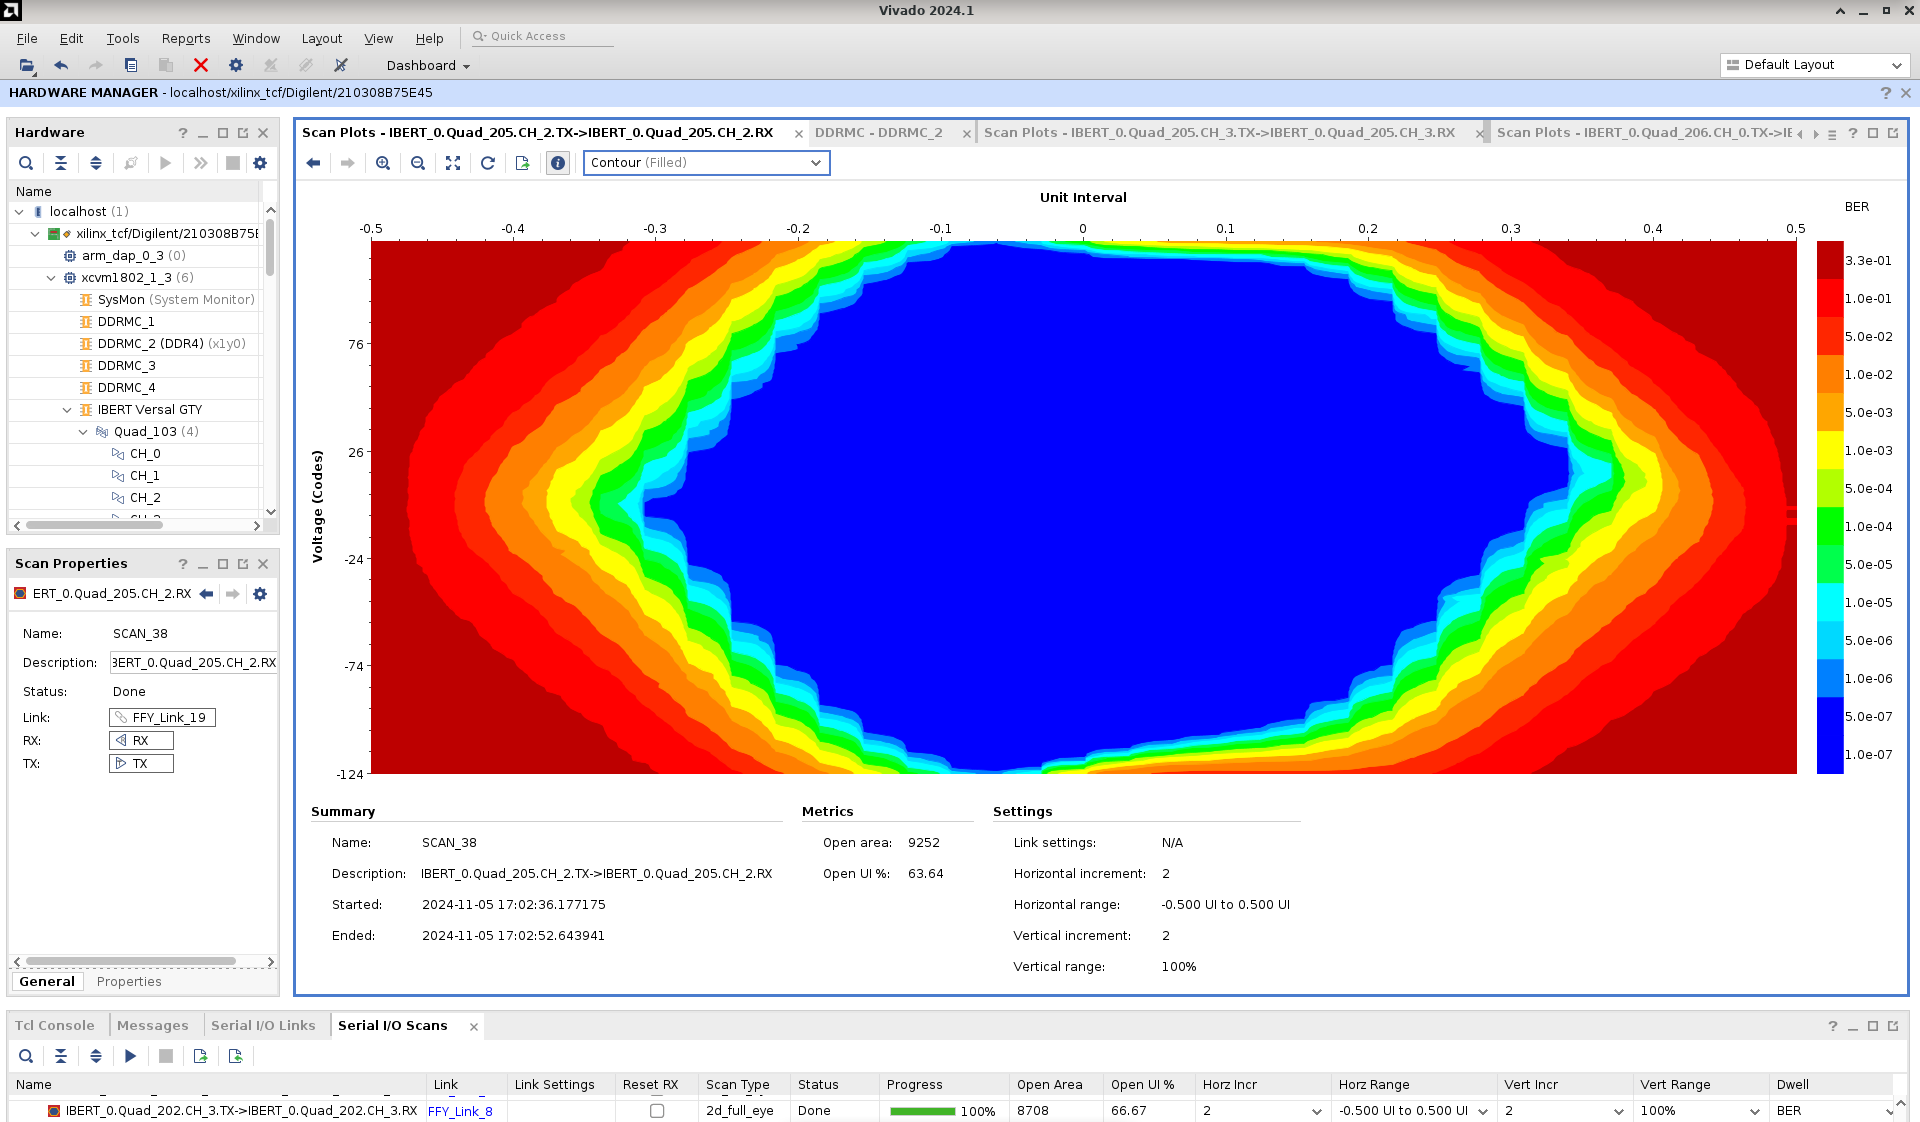
\includegraphics[width=\textwidth]{images/contributions/eyescan.png}
\caption[Sample of the eyescan of a GTY transceiver]{Sample of the eyescan of a GTY transceiver. Those transceivers receive the signals from the Firefly \protect\cite{firefly-optical-transceiver} modules and make them available to the FPGA. The GTY transceivers live inside the FPGA produced by AMD. This image represents the error rate of one transceiver. The blue part indicates a low error rate, while red indicates a high error rate\\
Y axis: the voltage received by the transceiver\\
X axis: Unit Intervals fractions, which essentially means that the signal is brought out of phase by a percentage of one clock cycle. A unit interval corresponds to a clock period.}
\label{fig:eyescan-test}
\end{figure}

\clearpage
\subsubsection{Challenges}

There is an official table listing the most critical discrete components on the \ac{PCB}; an excerpt is provided below in Table~\ref{tab:pcb-rail-measurements} (without excessive detail):

\begin{table}[H]
\centering
\caption[Reference value of resistors]{Key power rail sensor resistors and feedback impedance measurements for FLX-182-1B.}
\label{tab:pcb-rail-measurements}
\resizebox{\linewidth}{!}{%
\begin{tabular}{|l|l|l|l|l|}
\hline
\textbf{Module} & \textbf{RefDes} & \textbf{Power Rail} & \textbf{Sensor Resistor (Ohm)} & \textbf{Reference (Ohm)} \\
\hline
LTM4700 & U1  & VCCINT   & R884 1.0    & 1.0 \\
LTM4638 & U7  & MGTAVCC  & R940 12.2   & 12.2 \\
LTM4638 & U3  & MGTAVTT  & R934 278.2  & 278.2 \\
LTM4638 & U2  & SYS12    & R933 87.6   & 87.6 \\
LTM4638 & U4  & SYS15    & R935 194.9  & 194.9 \\
LTM4638 & U6  & SYS18    & R939 270.6  & 270.6 \\
LTM4638 & U5  & SYS33    & R936 101.9  & 101.9 \\
LTM4642 & U84 & SYS25    & R938 5.89k  & 5.89k \\
\hline
\end{tabular}%
}
\end{table}

\vspace{1em}

\begin{table}[ht]
\centering
\resizebox{\linewidth}{!}{%
\begin{tabular}{|l|l|l|l|}
\hline
\textbf{Power Rail} & \textbf{FB Impedance RefDes} & \textbf{Measured Impedance} & \textbf{Notes} \\
\hline
SYS38        & R937  & $\sim$300k    & Jumper resistors present \\
MGTVCCAUX    & R928  & 4.836k        & ADP124 U35 \\
DDR4 VTT     & R795  & 4.102k        & TPS51200 U58 \\
VCC5V        & R929  & 6.26k         & TPSM5601R5 U52 \\
VCC5VM       & R930  & 125.6         & U74 \\
\hline
\end{tabular}%
}
\caption{Power rail impedance measurements.}
\label{tab:impedance}
\end{table}

Due to the high density of components and their sizes, precisely locating them was challenging, and doing so consistently across different cards and production batches proved difficult. Furthermore, not all components needed the same type of inspection. Some discrete components required just visual inspection while other required one or more measurements. To help with the task, I developed a visual aid (Figure~\ref{fig:FLX-182-hardware-inspection} and ) to translate the tables into an image, thus streamlining the inspection process. Components were color-coded according to the type of inspection required.

\begin{figure}[H]
\centering
\begin{subfigure}[b]{\textwidth}
    \centering
    \includegraphics[width=\textwidth]{images/contributions/Resistors_front.jpg}
    \caption{Top view: FLX-182-1B color coded components to inspect.}
    \label{fig:FLX-182-top-resistors}
\end{subfigure}

\vspace{0.2cm}

\begin{subfigure}[b]{\textwidth}
    \centering
    \includegraphics[width=\textwidth]{images/contributions/Resistors_back.jpg}
    \caption{Bottom view: FLX-182-1B color coded components to inspect.}
    \label{fig:FLX-182-bot-resistors}
\end{subfigure}
\caption{FLX-182-1B hardware probing aid.}
\label{fig:FLX-182-hardware-inspection}
\end{figure}

A significant challenge involved isolating faults in malfunctioning cards. In two instances there was a blown capacitor, making those cases the easiest to diagnose. One notable issue arose with cards that failed to boot from the SD card, which was traced to a defect in the SD interface adapter.

Upon diagnosing the issues, I prepared detailed documentation to guide technicians in repairing the affected cards and replacing the faulty components.

Not all problem diagnosis was conducted independently; I collaborated with hardware engineers at \acf{BNL}.
